\documentclass[11pt]{article}

\usepackage{pdfsync}
\usepackage{amsmath}
% 1. Page Layout and Packages
\usepackage[left=0.25in,top=0.5in,right=0.25in,bottom=0.5in]{geometry} 
\usepackage{graphicx}
\usepackage[]{minted}
\usepackage{tcolorbox}


\usepackage{etoolbox}
\BeforeBeginEnvironment{minted}{\begin{tcolorbox}}%
\AfterEndEnvironment{minted}{\end{tcolorbox}}%

\usepackage{multicol} % Enables multiple columns for images in a row
\usepackage{caption}  % Allows captions outside of the figure environment

% 2. Image Path Setup
\graphicspath{{../codeScreenshots/}{../Problem4/}{../Problem2/}{../Problem3/}}

% 3. AUTOMATION: Custom command for compact BMPs in columns
% Usage: \bmpColImage{filename}{pixelWidth}{pixelHeight}{caption}
\newcommand{\bmpColImage}[4]{
\begin{figure}[H]
    \centering
        \includegraphics[width=\linewidth, natwidth=#2, natheight=#3]{#1}
        \captionof{figure}{#4}
        \small(#2 $\times$ #3 pixels)
    \end{figure}
}

\begin{document}

% Header Section
\noindent \textbf{Aron Rezene} \hfill \textbf{Image Processing: HW 1} \\
\noindent \today
\vspace{-5pt}
\vspace{1pt}   


\section{Code Structure}
Due to the increasing complexity of the project I have started a github repository as a way to keep track of the code. https://github.com/ahrgm5/imgPrcsng

Using object oriented data types, the project enables use of arbitrarily sized kernels, generic filters for both DFT \& DCT analysis. How most of this was achieved is well beyond the scope of the assignment focus so i will not explain much of how things work under the hood. 

\section{Assignment}


\subsection{Problem 1: Laplacian vs Unsharp Masking}
\subsubsection{Written Response}

In spatial image processing kernels are used to transform an image via convolution of the original image intensity with the kernel being used.

In unsharp masking, a blurred image is produced using an averaging kernel and is then subtracted from the original image. The blurred image, which has low frequency content, being removed from the image leaves mostly high frequency data. This is the mask that will scaled and reinserted in to the image. 

In laplacian sharpening the second derivative laplacian kernel extracts the edges in the image which are scaled an reinserted into the original image.

\begin{align*}
	\nabla ^{2} f &= \frac{\partial^{2} f}{\partial x^{2}} + \frac{\partial^{2} f}{\partial y^{2}} = -4f(x,y) + f(x-1,y) + f(x,y-1) + f(x+1,y) + f(x,y+1) \\
	I_{laplacian} &= I_{original} + k * \nabla ^{2} f(x,y) \\[1em]
	mask &= I_{original} - blurred \\ 
	I_{unsharp} &= I_{original} + k * mask
\end{align*}

Both implementations use a scaled difference operator to sharpen the original image.
  




\subsection{Problem 2:  Spatial Processing and Photo Enhancement }

\subsubsection{Part 1}

\begin{figure}[H]
	
\begin{minted}{c}
 BMPImage* pout = readBMP((src_images + "pout.bmp").c_str());
 if (pout) {
 BMPImage* pout_eq = apply_histogram_equalization(pout, plot, "Intensity Transformation u vs v");
 writeBMP((path + "Problem2/2.1/pout_equalized.bmp").c_str(), pout_eq);
 
  BMPImage* pout_stretched = apply_histogram_stretching(pout);
 writeBMP((path + "Problem2/2.1/pout_stretched.bmp").c_str(), pout_stretched);

 freeBMPImage(pout);
 freeBMPImage(pout_eq);
}

\end{minted}

\caption{Problem 2.1 section of main.cpp}
\label{figure:Problem2}
\end{figure}



\begin{multicols}{2}
	
	\bmpColImage{/2.1/pout_equalized.bmp}{240}{291}{Equalized Histogram Image}
	
	\bmpColImage{/2.1/pout_stretched.bmp}{240}{291}{Stretched Histogram Image}
	
	
	
\end{multicols}

These two images have distinct intensity profiles as a result of the different histogram techniques for altering the spread of intensity values. The following curve shows the transformation mapping the original pixel intensities to the intensities after equalization

\begin{multicols}{2}
	
	
		\begin{figure}[H]
		\centering
		
\includegraphics[width=\linewidth]{/2.1/transformation.png}
		\captionof{figure}{Equalized Histogram Intensity Transformation} 
	\end{figure}
	
	
	\begin{figure}[H]
		\centering
		
\includegraphics[width=\linewidth]{/2.1/transformation2.png}
		\captionof{figure}{Stretched Histogram Intensity Transformation} 
	\end{figure}

	
	
\end{multicols}




\subsubsection{Part 2}

\begin{figure}[H]
	
	\begin{minted}{c}

BMPImages leaf1, leaf2 ;
leaf1.count = 2; // Color & Grayscale
leaf2.count = 3; // Color, Resized & grayscale

leaf1.images = (BMPImage**)malloc(sizeof(BMPImage*) *leaf1.count);
leaf2.images = (BMPImage**)malloc(sizeof(BMPImage*) *leaf2.count);
leaf1.images[0] = readBMP((src_images + "leaf.bmp").c_str());
leaf2.images[0] = readBMP((src_images + "leaf2.bmp").c_str());

int w = leaf1.images[0]->info_header.width_px, h = leaf1.images[0]->info_header.height_px;

leaf2.images[1] = resize_bilinear(leaf2.images[0], w, h);
leaf1.images[1] = extract_channel_info(leaf1.images[0], 3, 1); 
leaf2.images[2] = extract_channel_info(leaf2.images[1], 3, 1);

if (leaf1.images) {
BMPImage* stretch = preprocess_for_edges(leaf1.images[0], 2.0f);
BMPImage* eq = apply_histogram_equalization(leaf1.images[0], plot, "Intensity Transformation");

// Laplacian Sharpening
BMPImages leaf_lap = sharpen_laplacian(leaf1.images[0], 1.0f, 3, 3);
BMPImages leaf_lap1 = sharpen_laplacian(stretch, 1.0f, 3, 3);
BMPImages leaf_lap2 = sharpen_laplacian(eq, 1.0f, 3, 3);
// Unsharp Masking
BMPImages leaf_unsharp = unsharp_masking(leaf1.images[0], 1.0f, 3, 3);
BMPImages leaf_unsharp1 = unsharp_masking(stretch, 1.0f, 3, 3);
BMPImages leaf_unsharp2 = unsharp_masking(eq, 1.0f, 3, 3);
	\end{minted}
	
	\caption{Problem 2.2 section of main.cpp}
	\label{figure:Problem2}
\end{figure}

In the second part we use the two different histogram techniques to prepare our image before applying the laplacian \& blurring kernel techniques for sharpening the image. Notice how multiple images can be stored together with th BMPIImages variable type. It makes it easier to switch between edited versions of an image. In this script the image was kept in color and was manipulated using RGB to HSI conversion.


\begin{multicols}{3}	 
	
	\bmpColImage{/2.2/laplacian/alpha_stretched_order1.bmp}{336}{343}{Stretched Image with Laplacian Sharpening }
	 \bmpColImage{/2.2/alpha_stretched.bmp}{336}{343}{Stretched Image}
	 
	 
	 \bmpColImage{/2.2/unsharp/alpha_stretched_order1.bmp}{336}{343}{Stretched Image with Unsharp Masking }
	 
	
\end{multicols}


\begin{multicols}{3}	 
	
	\bmpColImage{/2.2/laplacian/alpha_equalized_order1.bmp}{336}{343}{Equalized Image with Laplacian}

	\bmpColImage{/2.2/alpha_equalized.bmp}{336}{343}{Equalized Image}	
	
	\bmpColImage{/2.2/unsharp/alpha_equalized_order1.bmp}{336}{343}{Equalized Image with Unsharp Masking}

\end{multicols}

These histogram techniques before sharpening shrink the SNR ratio around 0-1 dB. Before the histogram techniques it was calculated that the SNR with the original image and MSE with the enhanced image given in the assignment turn out to be pretty good.




 

\subsection{Problem 3: High Frequency Filtering and Equalization}

\subsubsection{Code}
I was unable to use the ches xray image shown on the homework because I was unable to generate a safe bmp image (kept getting a corrupted file erro when loading into the program) so i used the same leaf image to evaluate the effects of changing the order of high pass filtering and equalization
\begin{figure}[H]
\begin{minted}{c}

BMPImage* test_img = readBMP((src_images + "leaf.bmp").c_str());
BMPImage* gray_test_img = extract_channel_info(test_img, 3, 1); // Convert to grayscale for frequency processing

if (test_img) {
int w = test_img->info_header.width_px;
int h = abs(test_img->info_header.height_px);
hpFilter* hp = (hpFilter*)create_filter(FILTER_DOMAIN_DFT, w, h, hpf_logic, sizeof(hpFilter));
hpf->sigma = std::max(w,h)/100;
	
// Order 1: High-Frequency Emphasis Filter -> Histogram Equalization
BMPImage* hpf_only = apply_frequency_filter_to_bmp(gray_test_img, (Filter*)hp);
BMPImage* order1 = apply_histogram_equalization(hpf_only, plot, "");
writeBMP((path + "Problem3/order1_hpf_then_histeq.bmp").c_str(), order1);

// Order 2: Histogram Equalization -> High-Frequency Emphasis Filter
BMPImage* eq_only = apply_histogram_equalization(gray_test_img, plot, "");
BMPImage* order2 = apply_frequency_filter_to_bmp(eq_only, (Filter*)gfltr);
writeBMP((path + "Problem3/order2_histeq_then_hpf.bmp").c_str(), order2);

destroy_filter((Filter*)hp);
freeBMPImage(test_img); freeBMPImage(hpf_only); freeBMPImage(order1);
freeBMPImage(eq_only); freeBMPImage(order2);
}
\end{minted}
\caption{Problem 3 section of main.cpp}
\label{figure:Extraction}
\end{figure}






\subsubsection{Results}

From the outputs shown on the next page it appears that histogram equalization. When the high frequency information is kept before equalization it we are essentially retuning the pixel values of the high frequency image data. This is order becomes useful when you want to preserve high frequency data. The second order looses of the original images data once the equalization occurs so it would be more useful in contrast is of greater concern in the image analysis.
\newpage
	 
\begin{multicols}{3}	 
	
	
	%\bmpColImage{order1_hpf_then_histeq.bmp}{336}{343}{Highpass filtering then Equalization }
		\begin{figure}[H]
	
		\includegraphics[width=\linewidth, natwidth = 336, natheight= 343]{order1_hpf_then_histeq.bmp}
		\captionof{figure}{Highpass Filtering then Equalization} 
		\end{figure}
		
	
	 		\begin{figure}[H]
	
		\includegraphics[width=\linewidth, natwidth = 336, natheight= 343]{gray_test.bmp}
		\captionof{figure}{Grayscale} 
		\end{figure}
		
				\begin{figure}[H]
	
		\includegraphics[width=\linewidth, natwidth = 336, natheight= 343]{order2_histeq_then_hpf.bmp}
		\captionof{figure}{Equalization then Highpass Filtering} 
		\end{figure}
	 %\bmpColImage{order2_histeq_then_hpf.bmp}{336}{343}{Equalization then highpass filtering}
	 
	
\end{multicols}

 




\subsection{Problem 4: DFT vs DCT \& Truncation }

\subsubsection{Code}

\begin{figure}[H]
\begin{minted}{c}
std::vector<std::string> task4_imgs = { "baboon.bmp", "monkeyking.bmp", "sunflower.bmp", "hex.bmp"};

        for (const std::string& img_name : task4_imgs) {
            std::cout << "Processing: " << img_name << "..." << std::endl;

            BMPImage* color_img = readBMP((src_images + img_name).c_str());
            if (!color_img) continue;

            // 4.1: Convert to Grayscale
            // (Assuming extract_channel_info(img, type, channel) extracts intensity)
            BMPImage* gray_img = extract_channel_info(color_img, 3, 1);

            // --- PREVENTING THE MEMORY ERROR ---
            // We store the strings in variables so they stay alive until the functions finish.
            std::string base = img_name.substr(0, img_name.find_last_of("."));

            std::string dft_title = "Centered DFT - " + img_name;
            std::string dft_spec_path = path + "Problem4/Spectrums/" + base + "_dft_spectrum.png";

            std::string dct_title = "Centered DCT - " + img_name;
            std::string dct_spec_path = path + "Problem4/Spectrums/" + base + "_dct_spectrum.png";

            // 4.1: Plot and Save 2D log magnitude
            run_dft_analysis(gray_img, dft_title.c_str(), plot, dft_spec_path.c_str());
            run_dct_analysis(gray_img, dct_title.c_str(), plot, dct_spec_path.c_str());

            // 4.2: Truncation Analysis (25% and 6.25%)
            double percentages[] = {0.25, 0.0625};
            std::string labels[] = {"quarter", "sixteenth"};
            int w = gray_img->info_header.width_px;
            int h = abs(gray_img->info_header.height_px);

            for (int i = 0; i < 2; i++) {
                // Setup Truncation Filters
TruncationFilter* tf_DFT = create_filter(FILTER_DOMAIN_DFT, w, h, rect_truncation_logic, sizeof(TruncationFilter));
                tf_DFT->percent = percentages[i];

TruncationFilter* tf_DCT = create_filter(FILTER_DOMAIN_DCT, w, h, rect_truncation_logic, sizeof(TruncationFilter));
                tf_DCT->percent = percentages[i];

                // Reconstruct Images
                BMPImage* recon_dft = apply_frequency_filter_to_bmp(gray_img, (Filter*)tf_DFT);
                BMPImage* recon_dct = apply_frequency_filter_to_bmp(gray_img, (Filter*)tf_DCT);

                // Compute SNR
                double snr_dft = calculate_snr(gray_img, recon_dft);
                double snr_dct = calculate_snr(gray_img, recon_dct);
printf("  [%s] Trunc: %.2f%% | DFT SNR: %.2f dB | DCT SNR: %.2f dB\n", img_name.c_str(), percentages[i]*100, snr_dft, snr_dct);

                // Organized Output Names
std::string dft_out = path + "Problem4/DFT_recon/" + base + "_recon_" + labels[i] + ".bmp";
std::string dct_out = path + "Problem4/DCT_recon/" + base + "_recon_" + labels[i] + ".bmp";

                writeBMP(dft_out.c_str(), recon_dft);
                writeBMP(dct_out.c_str(), recon_dct);

                // Cleanup Truncation
                destroy_filter((Filter*)tf_DFT); destroy_filter((Filter*)tf_DCT);
                freeBMPImage(recon_dft); freeBMPImage(recon_dct);
            }

            freeBMPImage(color_img);
            freeBMPImage(gray_img);
        }

\end{minted}

\caption{Problem 3 section of main.cpp}
\label{figure:Problem3}
\end{figure}


\subsubsection{Results}

Truncating the image to a smaller region in teh spectrum produces smoother images. The DCT centered plot shows the lack of symmetry due to the real basis of the transform.

Quarter truncated images show more detail than the sixteenth truncated images. 
\\

\begin{center}[H]
	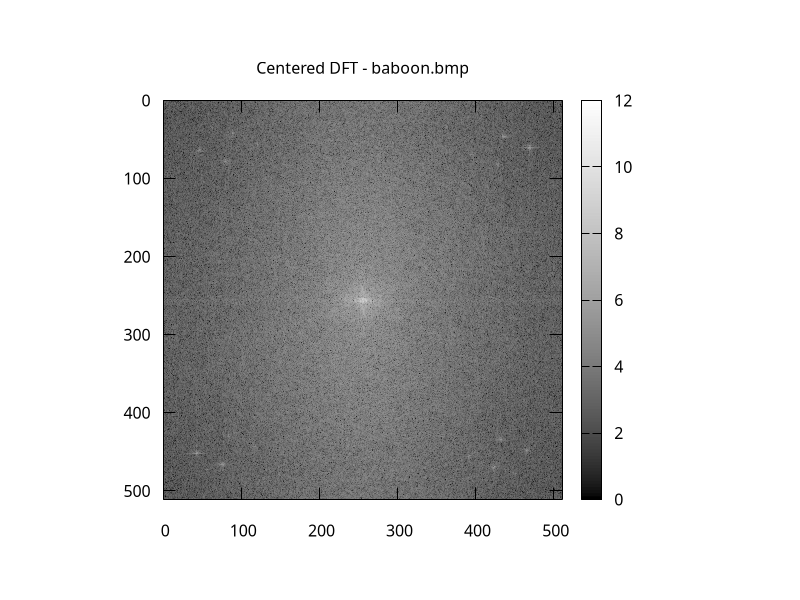
\includegraphics[width=\linewidth{4.2.png}
	\captionof{figure}{Sixteenth Truncated Low Pass Baboon Image with DCT} 
\end{center} 


\begin{multicols}{2} % Change '2' to the number of images you want in a row

				\begin{center}
		\includegraphics[width=\linewidth]{Spectrums/baboon_dft_spectrum.png}
		\captionof{figure}{  Baboon Image DFT } 
		\end{center}
		
	 	\begin{center}
		\includegraphics[width=\linewidth, natwidth = 512, natheight= 512]{DFT_recon/baboon_recon_quarter.bmp}
		\captionof{figure}{Quarter Truncated Low Pass Baboon Imagewith DFT} 
		\end{center}
		

	 	\begin{center}
		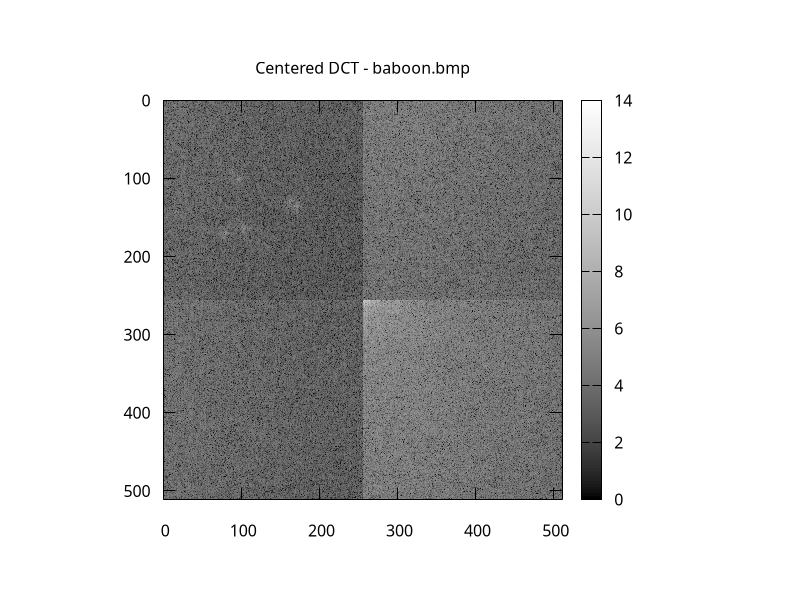
\includegraphics[width=\linewidth]{Spectrums/baboon_dct_spectrum.png}
		\captionof{figure}{  Baboon Image DCT } 
		\end{center}
		
		\begin{center}
		\includegraphics[width=\linewidth, natwidth = 512, natheight= 512]{DFT_recon/baboon_recon_sixteenth.bmp}
		\captionof{figure}{Sixteenth Truncated Low Pass Baboon Image with DFT} 
		\end{center}
	 		
 
		
		
	 	\begin{figure}[H]
		\includegraphics[width=\linewidth, natwidth = 512, natheight= 512]{DCT_recon/baboon_recon_quarter.bmp}
		\captionof{figure}{Quarter Truncated Low Pass Baboon Image with DCT} 
		\end{figure}
		
		\begin{figure}[H]
		\includegraphics[width=\linewidth, natwidth = 512, natheight= 512]{DCT_recon/baboon_recon_sixteenth.bmp}
		\captionof{figure}{Sixteenth Truncated Low Pass Baboon Image with DCT} 
		\end{figure} 
	 
\end{multicols}



  

\end{document}